\achapter{6}{Linear Dependence and Independence} \label{chap:independence}

\vspace*{-17 pt}
\framebox{
\parbox{\dimexpr\linewidth-3\fboxsep-3\fboxrule}
{\begin{fqs}
\item What are two ways to describe what it means for a set of vectors in $\R^n$ to be linearly independent? 
\item What are two ways to describe what it means for a set of vectors in $\R^n$ to be linearly dependent? 
\item If $S$ is a set of vectors, what do we mean by a basis for $\Span \ S$?
\item Given a nonzero set $S$ of vectors, how can we find a linearly independent subset of $S$ that has the same span as $S$?
\item How do we recognize if the columns of a matrix $A$ are linearly independent? 
\item How can we use a matrix to determine if a set $\{\vv_1, \vv_2, \ldots, \vv_k\}$ of vectors is linearly independent? 
\item How can we use a matrix to find a minimal spanning set for a set $\{\vv_1, \vv_2, \vv_3, \ldots, \vv_k\}$ of vectors in $\R^n$? 
\end{fqs}}}% \hspace*{3 pt}}

\vspace*{13 pt}

\csection{Application: B\'{e}zier Curves}
\label{sec:appl_bezier}

B\'{e}zier curves are simple curves that were first developed in 1959 by French mathematician Paul de Casteljau, who was working at the French automaker Citro\"{e}n. The curves were made public in 1962 by Pierre B\'{e}zier who used them in his work designing automobiles at the French car maker Renault. In addition to automobile design, B\'{e}zier curves have many other uses. Two of the most common applications of B\'{e}zier curves are font design and drawing tools. As an example, the letter ``S" in Palatino font is shown using B\'{e}zier curves in Figure \ref{F:Letter_S}. If you've used Adobe Illustrator, Photoshop, Macromedia Freehand, Fontographer, or any other of a number of drawing programs, then you've used B\'{e}zier curves. At the end of this section we will see how B\'{e}zier curves can be defined using linearly independent vectors and linear combinations of vectors.  
\begin{figure}[ht] \centering

\includegraphics{letter}
\caption{A letter $S$.}
\label{F:Letter_S}
\end{figure}


\csection{Introduction}
\label{sec:indep_intro}

In Section \ref{sec:vector_representation} we saw how to represent water-benzene-acetic acid chemical solutions with vectors, where the components represent the water, benzene and acid percentages.  We then considered a problem of determining if a given chemical solution could be made by mixing other chemical solutions. Suppose we now have three different water-benzene-acetic acid chemical solutions, one with 40\% water, 50\% benzene and 10\% acetic acid, the second with 52\% water, 42\% benzene and 6\% acid, and a third with 46\% water, 46\% benzene and 8\% acid. We represent the first chemical solution with the vector $\vv_1 = \left[ \begin{array}{c} 40\\50\\10\end{array} \right]$, the second with the vector $\vv_2 = \left[ \begin{array}{c} 52\\42\\6\end{array} \right]$, and the third with the vector $\vv_3 = \left[ \begin{array}{c} 46\\46\\8\end{array} \right]$. By combining these three chemical solutions we can make a chemical solution with 43\% water, 48\% benzene and 9\% acid as follows
\[\frac{7}{12}\vv_1 + \frac{1}{12} \vv_2 + \frac{1}{3}\vv_3 = \left[ \begin{array}{c} 43\\48\\9\end{array} \right].\]
However, if we had noticed that the third chemical solution can actually be made from the first two, that is,
\[\frac{1}{2}\vv_1 + \frac{1}{2} \vv_2 = \vv_3,\]
we might have realized that we don't need the third chemical solution to make the 43\% water, 48\% benzene and 9\% acid chemical solution. In fact, 
\[\frac{3}{4}\vv_1 + \frac{1}{4} \vv_2 = \left[ \begin{array}{c} 43\\48\\9\end{array} \right].\]
(See Exercise \ref{ex:1_d_acid} of Section \ref{sec:vector_representation}.) Using the third chemical solution (represented by $\vv_3$) uses more information than we actually need to make the desired 43\% water, 48\% benzene and 9\% acid chemical solution because the vector $\vv_3$ is redundant -- all of the material we need to make $\vv_3$ is contained in $\vv_1$ and $\vv_2$. This is the basic idea behind linear independence -- representing information in the most efficient way.

Information is often contained in and conveyed through vectors -- especially linear combinations of vectors. In this section we will investigate the concepts of linear dependence and independence of a set of vectors. Our goal is to be able to efficiently determine when a given set of vectors forms a \emph{minimal spanning set}. A minimal spanning set is a spanning set that contains the smallest number of vectors to obtain all of the vectors in the span. An important aspect of a minimal spanning set is that every vector in the span can be written in one and only one way as a linear combination of the vectors in the minimal spanning set. This will allow us to define the important notion of the dimension of a vector space. \\

\noindent \textbf{Review of useful information:} Recall that a linear combination of vectors $\vv_1$, $\vv_2$, $\ldots$, $\vv_k$ in $\R^n$ is a sum of scalar multiples of $\vv_1$, $\vv_2$, $\ldots$, $\vv_k$. That is, a linear combination of the vectors $\vv_1$, $\vv_2$, $\ldots$, $\vv_k$ is a vector of the form
\[c_1\vv_1 + c_2\vv_2 + \cdots + c_k\vv_k,\]
where $c_1$, $c_2$, $\ldots$, $c_k$ are scalars.

Recall also that the collection of all linear combinations of a set $\{\vv_1$, $\vv_2$, $\ldots$, $\vv_k\}$ of vectors in $\R^n$ is called the span of the set of vectors. That is, the span $\Span \{\vv_1, \vv_2, \ldots, \vv_k\}$ of the set $\vv_1$, $\vv_2$, $\ldots$, $\vv_k$ of vectors in $\R^n$ is the set
\[ \{c_1\vv_1 + c_2\vv_2 + \cdots + c_k\vv_k : \text{ where } c_1, c_2, \ldots, c_k \text{ are scalars}\}.\]

For example, a linear combination of vectors $\vv_1 = \left[ \begin{array}{c} 1\\1\\2 \end{array} \right]$ and $\vv_2 = \left[ \begin{array}{r} 0\\-2\\1 \end{array} \right]$ is $2 \vv_1-3\vv_2 = \left[ \begin{array}{c} 2\\8\\1 \end{array} \right]$. All linear combinations of these two vectors can be expressed as the collection of vectors of the form $\left[ \begin{array}{c} c_1\\c_1-2c_2\\2c_1+c_2 \end{array} \right]$ where $c_1, c_2$ are scalars. Suppose we want to determine whether $\vw=\left[ \begin{array}{c} 1\\2\\3 \end{array} \right]$ is in the span, in other words if $\vw$ is a linear combination of $\vv_1, \vv_2$. This means we are looking for $c_1, c_2$ such that 
\[  \left[ \begin{array}{c} c_1\\c_1-2c_2\\2c_1+c_2 \end{array} \right] = \left[ \begin{array}{c} 1\\2\\3 \end{array} \right] \, . \]
 we solve for the system represented with the augmented matrix 
\[ \left[\begin{array}{crc|c} 1&0&&1\\ 1&-2&&2 \\ 2&1&&3\end{array} \right] \,. \]
By reducing this matrix, we find that there are no solutions of the system, which implies that $\vw$ is not a linear combination of $\vv_1, \vv_2$. Note that we can use any names we please for the scalars, say $x_1, x_2$, if we prefer.



\begin{pa} \label{pa:1_f} Let $\vv_1 = \left[ \begin{array}{r} 2\\1\\-3 \end{array} \right]$, $\vv_2 =  \left[ \begin{array}{c} 1\\1\\0 \end{array} \right]$, and $\vv_3 = \left[ \begin{array}{r} 1\\-1\\-6 \end{array} \right]$, and let $\vb = \left[ \begin {array}{c} 0 \\ 1 \\ 3 \end {array} \right]$. If $\vb$ is in $\Span \{\vv_1, \vv_2, \vv_3\}$, we are interested in the most efficient way to represent $\vb$ as a linear combination of $\vv_1$, $\vv_2$, and $\vv_3$. 
\be
\item \label{act:PA1_f_1} The vector $\vb$ is in $\Span \{\vv_1, \vv_2, \vv_3\}$ if there exist $x_1$, $x_2$, and $x_3$ so that 
\[x_1 \vv_1 + x_2 \vv_2 + x_3 \vv_3 = \vb.\]
(Recall that we can use any letters we want for the scalars. They are simply unknown scalars we want to solve for.)
	\ba
	\item Explain why $\vb$ is in $\Span \{\vv_1, \vv_2, \vv_3\}$. (Hint: What is the matrix we need to reduce?) 


	\item Write $\vb$ as a linear combination of $\vv_1$, $\vv_2$, and $\vv_3$. In how many ways can $\vb$ be written as a linear combination of the vectors $\vv_1$, $\vv_2$, and $\vv_3$? Explain. 


	\ea



\item \label{act:PA1_f_2}  In problem \ref{act:PA1_f_1} we saw that the vector $\vb$ could be written in infinitely many different ways as linear combinations of $\vv_1$, $\vv_2$, and $\vv_3$. We now ask the question if we really need all of the vectors $\vv_1$, $\vv_2$, and $\vv_3$ to make $\vb$ as a linear combination in a unique way.  
	\ba
	\item Can the vector $\vb$ be written as a linear combination of the vectors $\vv_1$ and $\vv_2$? If not, why not? If so, in how many ways can $\vb$ be written as a linear combination of $\vv_1$ and $\vv_2$? Explain.


	\item If possible, write $\vb$ as a linear combination of $\vv_1$ and $\vv_2$.  


	\ea


\item In problem \ref{act:PA1_f_1} we saw that $\vb$ could be written in infinitely many different ways as a linear combination of the vectors $\vv_1$, $\vv_2$, and $\vv_3$. However, the vector $\vb$ could only be written in one way as a linear combination of $\vv_1$ and $\vv_2$. So $\vb$ is in $\Span \{\vv_1, \vv_2, \vv_3\}$ and $\vb$ is also in $\Span \{\vv_1, \vv_2\} $. This raises a question -- is \emph{any} vector in $\Span \{\vv_1, \vv_2, \vv_3\}$ also in $\Span\{\vv_1, \vv_2\}$. If so, then the vector $\vv_3$ is redundant in terms of forming the span of $\vv_1$, $\vv_2$, and $\vv_3$. For the sake of efficiency, we want to recognize and eliminate this redundancy.  
 
	\ba
	\item Can $\vv_3$ be written as a linear combination of the vectors $\vv_1$ and $\vv_2$? If not, why not? If so, write $\vv_3$ as a linear combination of $\vv_1$ and $\vv_2$. 
	
	
	\item Use the result of part (a) to decide if \emph{any} vector in $\Span\{\vv_1, \vv_2, \vv_3\}$ is also in $\Span\{\vv_1, \vv_2\}$. 


\ea

\ee

\end{pa}

\csection{Linear Independence}
\label{sec:lin_indep}

In this section we will investigate the concepts of linear dependence and independence of a set of vectors. Our goal is to be able to efficiently determine when a given set of vectors forms a \emph{minimal spanning set}. This will involve the concepts of span and linear independence. Minimal spanning sets are important in that they provide the most efficient way to represent vectors in a space, and will later allow us to define the dimension of a vector space.  


In Preview Activity \ref{pa:1_f} we considered the case where we had a set $\{\vv_1, \vv_2, \vv_3\}$ of three vectors, and the vector $\vv_3$ was in the span of $\{\vv_1, \vv_2\}$. So the the vector $\vv_3$ did not add anything to the span of $\{\vv_1, \vv_2\}$. In other words, the set $\{\vv_1, \vv_2, \vv_3\}$ was larger than it needed to be in order to generate the vectors in its span -- that is, $\Span\{\vv_1, \vv_2, \vv_3\} = \Span \{\vv_1, \vv_2\}$. However, neither of the vectors in the set $\{\vv_1, \vv_2\}$ could be removed without changing its span. In this case, the set $\{\vv_1, \vv_2\}$ is what we will call a \emph{minimal spanning set}\index{minimal spanning set} or a \emph{basis} for $\Span \ S$. There are two important properties that make $\{\vv_1, \vv_2\}$ a basis for $\Span \ S$. The first is that every vector in $\Span \ S$ can be written as linear combinations of $\vv_1$ and $\vv_2$ (we also use the terminology that the vectors $\vv_1$ and $\vv_2$ span $\Span \ S$), and the second is that every vector in $\Span \ S$ can be written in exactly one way as a linear combination of $\vv_1$ and $\vv_2$. This second property is the property of linear independence, and it is the property that makes the spanning set \emph{minimal}. 

To make a spanning set minimal, we want to be able to write every vector in the span in a unique way in terms of the spanning vectors. Notice that the zero vector can always be written as a linear combination of any set of vectors using 0 for all of the weights. So to have a \emph{minimal} or \emph{linearly independent} spanning set, that is, to have a unique representation for each vector in the span, it will need to be the case that the \emph{only} way we can write the zero vector as a linear combination of a set of vectors is if all of the weights are 0. This leads us to the definition of a linearly independent set of vectors.  


\begin{definition} \label{def:linear_independence_Rn} A set $\{\vv_1, \vv_2, \ldots, \vv_k\}$ of vectors in $\R^n$ is \textbf{linearly independent}\index{linear independence} if the vector equation
\[x_1 \vv_1 + x_2 \vv_2 + \cdots + x_k \vv_k = \vzero\]
for scalars $x_1, x_2, \ldots, x_k$ has only the trivial solution
\[x_1 = x_2 = x_3 = \cdots = x_k = 0.\]
If a set of vectors is not linearly independent, then the set is \textbf{linearly dependent}\index{linear dependence}.
\end{definition}

Alternatively, we say that the vectors $\vv_1, \vv_2, \ldots, \vv_k$ are linearly independent (or dependent) if the set $\{\vv_1, \vv_2, \ldots, \vv_k\}$ is linearly independent (or dependent).


Note that the definition tells us that a set $\{\vv_1, \vv_2, \ldots, \vv_k\}$ of vectors in $\R^n$ is linearly dependent if there are scalars $x_1$, $x_2$, $\ldots$, $x_n$, not all of which are 0 so that
\[x_1 \vv_1 + x_2 \vv_2 + \cdots + x_k \vv_k = \vzero.\]


\begin{activity} \label{act:1_f_1} Which of the following sets in $\R^2$ or $\R^3$ is linearly independent and which is linearly dependent? Why? For the linearly dependent sets, write one of the vectors as a linear combination of the others, if possible. 
\ba
\item $S_1 = \left\{\left[\begin{array}{c} 2 \\ 0 \\ 1 \end{array}\right], \left[\begin{array}{r} -2 \\ 8 \\ 1 \end{array}\right], \left[\begin{array}{r} -4 \\ 8 \\ 0 \end{array}\right]\right\}$.



\item $S_2 = \left\{\left[\begin{array}{c} 1 \\ 2 \\ 1 \end{array}\right], \left[\begin{array}{c} 0 \\ 2 \\ 3 \end{array}\right]\right\}$. (Hint: What relationship must exist between two vectors if they are linearly dependent?)



\item The vectors $\vu$, $\vv$, and $\vw$ as shown in Figure \ref{F:1_f_1}.
\begin{figure}[ht]
\begin{center}
\resizebox{!}{2.0in}{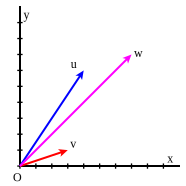
\includegraphics{1_f_lin_dependence}}
\caption{Vectors $\vu$, $\vv$, and $\vw$.}
\label{F:1_f_1}
\end{center}
\end{figure}


\ea

\end{activity}


Activity \ref{act:1_f_1} (a) and (c) illustrate how we can write one of the vectors in a linearly dependent set as a linear combination of the others. This would allow us to write at least one of the vectors in the span of the set in more than one way as a linear combination of vectors in this set. We prove this result in general in the following theorem.

\begin{theorem} \label{thm:Dependence} A set $\{\vv_1, \vv_2, \ldots, \vv_k\}$ of vectors in $\R^n$ is linearly dependent if and only if at least one of the vectors in the set can be written as a linear combination of the remaining vectors in the set.
\end{theorem}

The next activity is intended to help set the stage for the proof of Theorem \ref{thm:Dependence}. 

\begin{activity} \label{act:1_f_1b} The statement of Theorem \ref{thm:Dependence} is a bi-conditional statement (an if and only if statement). To prove this statement about the set $S$ we need to show two things about $S$. One: we must demonstrate that if $S$ is a linearly dependent set, then at least one vector in $S$ is a linear combination of the other vectors (this is the ``only if" part of the biconditional statement) and Two: if at least one vector in $S$ is a linear combination of the others, then $S$ is linearly dependent (this is the ``if" part of the biconditional statement). We illustrate the main idea of the proof using a three vector set $S = \{\vv_1, \vv_2, \vv_3\}$. 
	\ba
	\item First let us assume that $S$ is a linearly dependent set and show that at least one vector in $S$ is a linear combination of the other vectors. Since $S$ is linearly dependent we can write the zero vector as a linear combination of $\vv_1$, $\vv_2$, and $\vv_3$ with at least one nonzero weight. For example, suppose 
\begin{equation} \label{eq:1_f_dependence_thm_1}
2\vv_1 + 3\vv_2 + 4\vv_3 = \vzero.
\end{equation}
Solve Equation (\ref{eq:1_f_dependence_thm_1}) for the vector $\vv_2$ to show that $\vv_2$ can be written as a linear combination of $\vv_1$ and $\vv_3$. Conclude that $\vv_2$ is a linear combination of the other vectors in the set $S$. 

	\item Now we assume that at least one of the vectors in $S$ is a linear combination of the others. For example, suppose that
\begin{equation} \label{eq:1_f_dependence_thm_2}
 \vv_3 = \vv_1 + 5\vv_2.
\end{equation}
Use vector algebra to rewrite Equation \ref{eq:1_f_dependence_thm_2} so that $\vzero$ is expressed as a linear combination of $\vv_1$, $\vv_2$, and $\vv_3$ such that the weight on $\vv_3$ is not zero. Conclude that the set $S$ is linearly dependent. 

	\ea
	
\end{activity}

Now we provide a formal proof of Theorem \ref{thm:Dependence}, using the ideas from Activity \ref{act:1_f_1b}.

\begin{proof}[Proof of Theorem \ref{thm:Dependence}] Let $S = \{\vv_1, \vv_2, \ldots, \vv_k\}$ be a set of vectors in $\R^n$.  We will begin by verifying the first statement.

We assume that $S$ is a linearly dependent set and show that at least one vector in $S$ is a linear combination of the others. Since $S$ is linearly dependent, there are scalars $x_1$, $x_2$, $\ldots$, $x_n$, not all of which are 0, so that 
\begin{equation} \label{eq:1_f_dependence_1} 
x_1\vv_1 + x_2\vv_2 + \cdots +  x_{k}\vv_{k} = \vzero.
\end{equation}
We don't know which scalar(s) are not zero, but there is at least one. So let us assume that $x_i$ is not zero for some $i$ between 1 and $k$.  We can then subtract $x_i \vv_i$ from both sides of Equation (\ref{eq:1_f_dependence_1}) and divide by $x_i$ to obtain
\[\vv_i = \frac{x_1}{x_i}\vv_1 + \frac{x_2}{x_i}\vv_2 + \cdots + \frac{x_{i-1}}{x_i}\vv_{i-1} +  \frac{x_{i+1}}{x_i}\vv_{i+1} + \frac{x_{i+2}}{x_i}\vv_{i+2} + \cdots + \frac{x_{k}}{x_i}\vv_{k}.\]
Thus, the vector $\vv_i$ is a linear combination of $\vv_1$, $\vv_2$, $\ldots$, $\vv_{i-1}$, $\vv_{i+1}$, $\ldots$, $\vv_k$, and at least one of the vectors in $S$ is a linear combination of the other vectors in $S$. 

To verify the second statement, we assume that at least one of the vectors in $S$ can be written as a linear combination of the others and show that $S$ is then a linearly dependent set. We don't know which vector(s) in $S$ can be written as a linear combination of the others, but there is at least one. Let us suppose that $\vv_i$ is a linear combination of the vectors $\vv_1$, $\vv_2$, $\ldots$, $\vv_{i-1}$, $\vv_{i+1}$, $\ldots$, $\vv_k$ for some $i$ between 1 and $k$. Then there exist scalars  $x_1$, $x_2$, $\ldots$, $x_{-1}$, $x_{i+1}$, $\ldots$, $x_n$ so that 
\[\vv_i = x_1\vv_1 + x_2\vv_2 + \cdots + x_{i-1}\vv_{i-1} +  x_{i+1}\vv_{i+1} + x_{i+2}\vv_{i+2} + \cdots + x_{k}\vv_{k}.\]
It follows that 
\[\vzero = x_1\vv_1 + x_2\vv_2 + \cdots + x_{i-1}\vv_{i-1} +  (-1)\vv_i + x_{i+1}\vv_{i+1} + x_{i+2}\vv_{i+2} + \cdots + x_{k}\vv_{k}.\] 
So there are scalars there are scalars $x_1$, $x_2$, $\ldots$, $x_n$ (with $x_i = -1$), not all of which are 0, so that 
\[x_1\vv_1 + x_2\vv_2 + \cdots +  x_{k}\vv_{k} = \vzero.\]
This makes $S$ a linearly dependent set. 
\end{proof}

With a linearly dependent set, at least one of the vectors in the set is a linear combination of the others. With a linearly independent set, this cannot happen -- no vector in the set can be written as a linear combination of the others. This result is given in the next theorem. You may be able to see how Theorems \ref{thm:Dependence} and \ref{thm:Independence} are logically equivalent.  


\begin{theorem} \label{thm:Independence} A set $\{\vv_1, \vv_2, \ldots, \vv_k\}$ of vectors in $\R^n$ is linearly independent if and only if no vector in the set can be written as a linear combination of the remaining vectors in the set.
\end{theorem}


\begin{activity} \label{act:1_f_2}  As was hinted at in Preview Activity \ref{pa:1_f}, an important consequence of a linearly independent set is that every vector in the span of the set can be written in one and only one way as a linear combination of vectors in the set. It is this uniqueness that makes linearly independent sets so useful. We explore this idea in this activity for a linearly independent set of three vectors. Let $S = \{\vv_1, \vv_2, \vv_3\}$ be a linearly independent set of vectors in $\R^n$ for some $n$, and let $\vb$ be a vector in $\Span \ S$. To show that $\vb$ can be written in exactly one way as a linear combination of vectors in $S$, we assume that 
\[\vb = x_1 \vv_1 + x_2 \vv_2 + x_3 \vv_3 \ \ \text{ and } \ \ \vb = y_1\vv_1 + y_2 \vv_2 + y_3 \vv_3\]
for some scalars $x_1$, $x_2$, $x_3$, $y_1$, $y_2$, and $y_3$. We need to demonstrate that $x_1=y_1$, $x_2=y_2$, and  $x_3=y_3$. 
	\ba
	\item Use the two different ways of writing $\vb$ as a linear combination of $\vv_1, \vv_2$ and $\vv_3$ to come up with a linear combination expressing $\vzero$ as a linear combination of these vectors.	
	
	\item Use the linear independence of the vectors $\vv_1, \vv_2$ and $\vv_3$ to explain why $x_1=y_1$, $x_2=y_2$, and  $x_3=y_3$.
	
	\ea
\end{activity}



Activity \ref{act:1_f_2} contains the general ideas to show that any vector in the span of a linearly independent set can be written in one and only one way as a linear combination of the vectors in the set. The weights of such a linear combination provide us a \emph{coordinate system} for the vectors in terms of the basis. Two familiar examples of coordinate systems are the Cartesian coordinates in the $xy$-plane, and $xyz$-space. We will revisit the coordinate system idea in a later chapter. 

In the next theorem we state and prove the general case of any number of linearly independent vectors producing unique representations as linear combinations.



\begin{theorem} \label{thm:1_f_unique_representation} Let $S = \{\vv_1, \vv_2, \ldots, \vv_k\}$ be a linearly independent set of vectors in $\R^n$. Any vector in $\Span \ S$ can be written in one and only one way as a linear combination of the vectors $\vv_1$, $\vv_2$, $\ldots$, $\vv_k$.  
\end{theorem}

\begin{proof} Let $S = \{\vv_1, \vv_2, \ldots, \vv_k\}$ be a linearly independent set of vectors in $\R^n$, and let $\vb$ be a vector in $\Span \ S$. By definition, it follows that $\vb$ can be written as a linear combination of the vectors in $S$. It remains for us to show that this representation is unique. So assume that 
\begin{equation} \label{eq:1_f_1} 
\vb = x_1 \vv_1 + x_2 \vv_2 + \cdots + x_k \vv_k \ \ \text{ and } \ \ \vb = y_1\vv_1 + y_2 \vv_2 + \cdots + y_k \vv_k
\end{equation}
for some scalars $x_1$, $x_2$, $\ldots$, $x_k$, and $y_1$, $y_2$, $\ldots$, $y_k$. Then 
\[x_1 \vv_1 + x_2 \vv_2 + \cdots + x_k \vv_k = y_1\vv_1 + y_2 \vv_2 + \cdots + y_k \vv_k.\]
Subtracting all terms from the right side and using a little vector algebra gives us 
\[(x_1-y_1) \vv_1 + (x_2-y_2) \vv_2 + \cdots + (x_k-y_k) \vv_k = \vzero.\]
 The fact that $S$ is a linearly independent set implies that 
 \[x_1-y_1=0, \ x_2-y_2 = 0, \ \ldots, \ x_k-y_k=0,\]
showing that $x_i=y_i$ for every $i$ between 1 and $k$. We conclude that the representation of $\vb$ as a linear combination of the linearly independent vectors in $S$ is unique. 

\end{proof}


\csection{Determining Linear Independence}
\label{sec:determ_lin_ind}

The definition and our previous work give us a straightforward method for determining when a set of vectors in $\R^n$ is linearly independent or dependent.  



\begin{activity} \label{act:1_f_3} In this activity we learn how to use a matrix to determine in general if a set of vectors in $\R^n$ is linearly independent or dependent. Suppose we have $k$ vectors $\vv_1$, $\vv_2$, $\ldots$, $\vv_k$ in $\R^n$. To see if these vectors are linearly independent, we need to find the solutions to the vector equation
\begin{equation} \label{eq:lin_indep}
x_1 \vv_1 + x_2 \vv_2 + \cdots + x_k \vv_k = \vzero.
\end{equation}
If we let $A = [\vv_1 \  \vv_2 \ \vv_3 \ \cdots \ \vv_k]$ and $\vx = \left[ \begin{array}{c} x_1 \\ x_2 \\ \vdots \\ x_k \end{array} \right]$, then we can write the vector equation (\ref{eq:lin_indep}) in matrix form $A \vx = \vzero$. Let $B$ be the reduced row echelon form of $A$.
	\ba
	\item  What can we say about the pivots of $B$ in order for $A \vx = \vzero$ to have exactly one solution? Under these conditions, are the vectors $\vv_1$, $\vv_2$, $\ldots$, $\vv_k$ linearly independent or dependent? 

	
	
	\item What can we say about the rows or columns of $B$ in order for $A \vx = \vzero$ to have infinitely many solutions? Under these conditions, are the vectors $\vv_1$, $\vv_2$, $\ldots$, $\vv_k$ linearly independent or dependent? 
	
	
	
	\item Use the result of parts (a) and (b) to determine if the vectors $\vv_1 = \left[ \begin{array}{r} 1 \\ -1 \\ 2 \\ 0 \end{array} \right]$, $\vv_2 = \left[ \begin{array}{c} 1 \\ 0 \\ 2 \\ 3 \end{array} \right]$, and $\vv_3 = \left[ \begin{array}{c} 0 \\ 0 \\ 2 \\ 1 \end{array} \right]$ in $\R^4$ are linearly independent or dependent. If dependent, write one of the vectors as a linear combination of the others. You may use the fact that the matrix $\left[ \begin{array}{rcc} 1&1&0 \\ -1&0&0 \\ 2&2&2 \\ 0&3&1 \end{array} \right]$ is row equivalent to $\left[ \begin{array}{rcc} 1&0&0 \\ 0&1&0 \\ 0&0&1 \\ 0&0&0 \end{array} \right]$.



\ea

\end{activity}

\csection{Minimal Spanning Sets}
\label{sec:min_span_set}

It is important to note the differences and connections between linear independence, span, and minimal spanning set. 
\begin{itemize}
\item The set $S = \left\{ \left[ \begin{array}{c} 1 \\ 0 \\ 0 \end{array} \right], \left[ \begin{array}{c} 0 \\ 1 \\ 0 \end{array} \right] \right\}$ is not a minimal spanning set for $\R^3$ even though $S$ is a linearly independent set. Note that $S$ does not span $\R^3$ since the vector $\left[ \begin{array}{c} 0 \\ 0 \\ 1 \end{array} \right] $ is not in $\Span \ S$. 
\item The set $T = \left\{ \left[ \begin{array}{c} 1 \\ 0 \\ 0 \end{array} \right], \left[ \begin{array}{c} 0 \\ 1 \\ 0 \end{array} \right] , \left[ \begin{array}{c} 0 \\ 0 \\ 1 \end{array} \right] , \left[ \begin{array}{c} 1 \\ 1 \\ 1 \end{array} \right] \right\}$ is not a minimal spanning set for $\R^3$ even though $\Span \ T = \R^3$. Note that 
\[\left[ \begin{array}{c} 1 \\ 1 \\ 1 \end{array} \right] = \left[ \begin{array}{c} 1 \\ 0 \\ 0 \end{array} \right] + \left[ \begin{array}{c} 0 \\ 1 \\ 0 \end{array} \right] + \left[ \begin{array}{c} 0 \\ 0 \\ 1 \end{array} \right], \]
so $T$ is not a linearly independent set.
\item The set $U = \left\{ \left[ \begin{array}{c} 1 \\ 0 \\ 0 \end{array} \right], \left[ \begin{array}{c} 0 \\ 1 \\ 0 \end{array} \right] , \left[ \begin{array}{c} 0 \\ 0 \\ 1 \end{array} \right]  \right\}$ is a minimal spanning set for $\R^3$ since it satisfies both characteristics of a minimal spanning set: $\Span \ U = \R^3$ AND $U$ is linearly independent. 
\end{itemize}
The three concepts -- linear independence, span, and minimal spanning set -- are different. The important point to note is that minimal spanning set must be both linearly independent and span the space. 

To find a minimal spanning set we will often need to find a smallest subset of a given set of vectors that has the same span as the original set of vectors. In this section we determine a method for doing so. 

\begin{activity} \label{act:1_f_4} Let $\vv_1 = \left[ \begin{array}{r} -1 \\ 0 \\ 2 \end{array} \right]$, $\vv_2 = \left[ \begin{array}{r} 2 \\ 0 \\ -4 \end{array} \right]$, $\vv_3 = \left[ \begin{array}{c} 0 \\ 1 \\ 3 \end{array} \right]$, and $\vv_4 = \left[ \begin{array}{r} -3 \\ 4 \\ 18 \end{array} \right]$ in $\R^3$. Assume that the reduced row echelon form of the matrix $A = \left[ \begin{array}{rrcr} -1&2&0&-3 \\ 0&0&1&4 \\ 2&-4&3&18 \end{array} \right]$ is $\left[ \begin{array}{crcc} 1&-2&0&3 \\ 0&0&1&4 \\ 0&0&0&0 \end{array} \right]$. 
	\ba
	\item Write the general solution to the homogeneous system $A \vx = \vzero$, where $\vx = \left[ \begin{array}{c} x_1 \\ x_2 \\ x_3 \\ x_4 \end{array} \right]$. Write all linear combinations of $\vv_1$, $\vv_2$, $\vv_3$, and $\vv_4$ that are equal to $\vzero$, using weights that only involve $x_2$ and $x_4$. 
	
	
	
	\item Explain how we can conveniently choose the weights in the general solution to $A \vx = \vzero$ to show that the vector $\vv_4$ is a linear combination of $\vv_1$, $\vv_2$, and $\vv_3$. What does this tell us about $\Span \{\vv_1, \vv_2, \vv_3\}$ and $\Span \{\vv_1, \vv_2, \vv_3, \vv_4\}$? 
	
	
	
	\item Explain how we can conveniently choose the weights in the general solution to $A \vx = \vzero$ to show why the vector $\vv_2$ is a linear combination of $\vv_1$ and $\vv_3$. What does this tell us about $\Span \{\vv_1, \vv_3\}$ and $\Span \{\vv_1, \vv_2, \vv_3 \}$?
	
	
	
	\item Is $\{\vv_1, \vv_3\}$ a minimal spanning set for $\Span \{\vv_1, \vv_2, \vv_3, \vv_4\}$? Explain your response. 
	
	
	
	
	\ea
\end{activity}



Activity \ref{act:1_f_4} illustrates how we can use a matrix to determine a minimal spanning set for a given set of vectors $\{\vv_1, \vv_2, \ldots, \vv_k\}$ in $\R^n$.
\begin{itemize}
\item Form the matrix $A = [\vv_1 \ \vv_2 \ \cdots \ \vv_k]$.
\item Find the reduced row echelon form $[B \ | \ \vzero]$ of $[A \ | \ \vzero]$. If $B$ contains non-pivot columns, say for example that the $i$th column is a non-pivot column, then we can choose the weight $x_i$ corresponding to the $i$th column to be 1 and all weights corresponding to the other non-pivot columns to be 0 to make a linear combination of the columns of $A$ that is equal to $\vzero$. This allows us to write $\vv_i$ as a linear combination of the vectors corresponding to the pivot columns of $A$ as we did in the proof of Theorem \ref{thm:Independence}. So every vector corresponding to a non-pivot column is in the span of the set of vectors corresponding to the pivot columns. The vectors corresponding to the pivot columns are linearly independent, since the matrix with those columns has every column as a pivot column. Thus, the set of vectors corresponding to the pivot columns of $A$ forms a minimal spanning set for $\{\vv_1, \vv_2, \ldots, \vv_k\}$.
\end{itemize}

\noindent \textbf{IMPORTANT NOTE!} The set of pivot columns of the reduced row echelon form of $A$ will normally not have the same span as the set of columns of $A$, so it is critical that we use columns of $A$, NOT $B$ in our minimal spanning set.



\begin{activity} \label{act:1_f_5} Find a minimal spanning set for the span of the set 
\[\left\{ \left[ \begin{array}{c} 1 \\ 1 \\ 0 \\ 0 \end{array} \right], \left[ \begin{array}{c} 2 \\ 3 \\ 0 \\ 0 \end{array} \right], \left[ \begin{array}{c} 0 \\ 1 \\ 2 \\ 0 \end{array} \right], \left[ \begin{array}{c} 4 \\ 1 \\ 0 \\ 0 \end{array} \right] \right\}.\] 



\end{activity}

Activity \ref{act:1_f_4} also illustrates a general process by which we can find a minimal spanning set -- that is the smallest subset of vectors that has the same span. This process will be useful later when we consider vectors in arbitrary vector spaces. The idea is that if we can write one of the vectors in a set $S$ as a linear combination of the remaining vectors, then we can remove that vector from the set and maintain the same span. In other words, begin with the span of a set $S$ and follow these steps:
\begin{description}
\item[Step 1.] If $S$ is a linearly independent set, we already have a minimal spanning set.
\item[Step 2.] If $S$ is not a linearly independent set, then one of the vectors in $S$ is a linear combination of the others. Remove that vector from $S$ to obtain a new set $T$. It will be the case that $\Span \ T = \Span \ S$.
\item[Step 3.] If $T$ is a linearly independent set, then $T$ is a minimal spanning set. If not, repeat steps 2 and 3 for the set $T$ until you arrive at a linearly independent set.
\end{description}
This process is guaranteed to stop as long as the set contains at least one nonzero vector. A verification of the statement in Step 2 that $\Span \ T = \Span \ S$ is given in the next theorem.



\begin{theorem} \label{thm:minimal_spanning_set} Let $\{\vv_1, \vv_2, \ldots, \vv_k\}$ be a set of vectors in $\R^n$ so that for some $i$ between 1 and $k$, $\vv_i$ is in $\Span \{\vv_1, \vv_2, \ldots, \vv_{i-1}, \vv_{i+1}, \ldots, \vv_k\}$. Then
\[\Span \{\vv_1, \vv_2, \ldots, \vv_k\} = \Span \{\vv_1, \vv_2, \ldots, \vv_{i-1}, \vv_{i+1}, \ldots, \vv_k\}.\]
\end{theorem}



\begin{proof} Let $\{\vv_1, \vv_2, \ldots, \vv_k\}$ be a set of vectors in $\R^n$ so that $\vv_i$ is in the span of $\vv_1$, $\vv_2$, $\ldots$, $\vv_{i-1}$, $\vv_{i+1}$, $\ldots$, and $\vv_k$ for some $i$ between 1 and $k$. To show that 
\[\Span \{\vv_1, \vv_2, \ldots, \vv_k\} = \Span \{\vv_1,  \ldots, \vv_{i-1}, \vv_{i+1}, \ldots, \vv_k\},\]
we need to show that
\begin{enumerate}
\item every vector in $\Span \{\vv_1, \vv_2, \ldots, \vv_k\}$ is in $\Span\{\vv_1, \ldots, \vv_{i-1}, \vv_{i+1}, \ldots, \vv_k\}$, and
\item every vector in $\Span \{\vv_1,  \ldots, \vv_{i-1}, \vv_{i+1}, \ldots, \vv_k\}$ is in \\ $\Span \{\vv_1, \ldots, \vv_k\}$.
\end{enumerate}
Let us consider the second containment. Let $\vx$ be a vector in the span of $\vv_1$, $\vv_2$, $\ldots$, $\vv_{i-1}$, $\vv_{i+1}$, $\ldots$, and $\vv_k$. Then
\[\vx = x_1\vv_1 + x_2\vv_2 + \cdots + x_{i-1}\vv_{i-1} + x_{i+1}\vv_{i+1} + \cdots + x_k\vv_k\]
for some scalars $x_1$, $x_2$, $\ldots$, $x_{i-1}$, $x_{i+1}$, $\ldots$, $x_k$. Note that
\[\vx = x_1\vv_1 + x_2\vv_2 + \cdots + x_{i-1}\vv_{i-1} + (0)\vv_i + x_{i+1}\vv_{i+1} + \cdots + x_k\vv_k\]
as well, so $\vx$ is in $\Span \{\vv_1, \vv_2, \ldots, \vv_k\}$. Thus, 
\[\Span \{\vv_1, \vv_2, \ldots, \vv_{i-1}, \vv_{i+1}, \ldots, \vv_k\} \subseteq  \Span \{\vv_1, \vv_2, \ldots, \vv_k\}.\]
(This same argument shows a more general statement that if $S$ is a subset of $T$, then $\Span \ S \subseteq \Span \ T$.)

Now we demonstrate the first containment. Here we need the assumption that $\vv_i$ is in $\Span \{\vv_1$, $\vv_2$, $\ldots$, $\vv_{i-1}$, $\vv_{i+1}$, $\ldots$, $\vv_k\}$ for some $i$ between 1 and $k$. That assumption gives us 
\begin{equation} \label{eq:lin_depend_containment}
\vv_i = c_1 \vv_1 + c_2\vv_2 + \cdots + c_{i-1}\vv_{i-1} + c_{i+1}\vv_{i+1} + \cdots + c_k\vv_k
\end{equation}
for some scalars $c_1$, $c_2$, $\ldots$, $c_{i-1}$, $c_{i+1}$, $\ldots$, $c_k$. Now let $\vx$ be a vector in the span of $\vv_1$, $\vv_2$, $\ldots$, $\vv_k$. Then
\[\vx = x_1\vv_1 + x_2\vv_2 + \cdots + x_k\vv_k\]
for some scalars $x_1$, $x_2$, $\ldots$, $x_k$. Substituting from (\ref{eq:lin_depend_containment}) shows that 
\begin{align*}
\vx &= x_1\vv_1 + x_2\vv_2 + \cdots + x_k\vv_k \\
	&= x_1\vv_1 + x_2\vv_2 + \cdots + x_{i-1} \vv_{i-1} + x_i \vv_i + x_{i+1}\vv_{i+1} + \cdots + x_k\vv_k \\
	&= x_1\vv_1 + x_2\vv_2 + \cdots + x_{i-1} \vv_{i-1} \\
	&\qquad + x_i[c_1 \vv_1 + c_2\vv_2 + \cdots + c_{i-1}\vv_{i-1} + c_{i+1}\vv_{i+1} + \cdots + c_k\vv_k]  \\
	&\qquad + x_{i+1}\vv_{i+1} + \cdots + x_k\vv_k \\
	&= (x_1+x_ic_1)\vv_1 + (x_2+x_ic_2)\vv_2 + \cdots + (x_{i-1}+x_ic_{i-1}) \vv_{i-1} \\
	&\qquad + (x_{i+1}+x_ic_{i+1}) \vv_{i+1} \cdots + (x_k+x_ic_k)\vv_k.
\end{align*}
So $\vx$ is in $\Span \{\vv_1, \vv_2, \ldots, \vv_{i-1}, \vv_{i+1}, \ldots, \vv_k\}$ and 
\[\Span \{\vv_1, \vv_2, \ldots, \vv_k\} \subseteq \Span \{\vv_1, \vv_2, \ldots, \vv_{i-1}, \vv_{i+1}, \ldots, \vv_k\}.\]
 Since the two sets are subsets of each other, they must be equal sets. We conclude that
\[\Span \{\vv_1, \vv_2, \ldots, \vv_k\} = \Span \{\vv_1, \vv_2, \ldots, \vv_{i-1}, \vv_{i+1}, \ldots, \vv_k\}.\]
\end{proof}



The result of Theorem \ref{thm:minimal_spanning_set} is that if we have a finite set $S$ of vectors in $\R^n$, we can eliminate those vectors that are linear combinations of others until we obtain a smallest set of vectors that still has the same span. As mentioned earlier, we call such a minimal spanning set a basis.



\begin{definition} \label{def:1_f_basis} Let $S$ be a set of vectors in $\R^n$. A subset $B$ of $S$ is a \textbf{basis}\index{basis} for $\Span \ S$ if $B$ is linearly independent and $\Span \ B = \Span \ S$. 
\end{definition}



\noindent \textbf{IMPORTANT NOTE: } A basis is defined by two characteristics. A basis must span the space in question and a basis must be a linearly independent set. It is the linear independence that makes a basis a \emph{minimal} spanning set. 

We have worked with a familiar basis in $\R^2$ throughout our mathematical careers. A vector $\left[ \begin{array}{c} a \\ b \end{array} \right]$ in $\R^2$ can be written as 
\[\left[ \begin{array}{c} a \\ b \end{array} \right] = a\left[ \begin{array}{c} 1 \\ 0 \end{array} \right] + b\left[ \begin{array}{c} 0 \\ 1 \end{array} \right].\]
So the set $\{\ve_1, \ve_2\}$, where $\ve_1 = \left[ \begin{array}{c} 1 \\ 0 \end{array} \right]$ and $\ve_2 = \left[ \begin{array}{c} 0 \\ 1 \end{array} \right]$ spans $\R^2$. Since the columns of $[\ve_1 \ \ve_2]$ are linearly independent, so is the set $\{\ve_1, \ve_2\}$. Therefore, the set $\{\ve_1, \ve_2\}$ is a basis for $\R^2$. The vector $\ve_1$ is in the direction of the positive $x$-axis and the vector $\ve_2$ is in the direction of the positive $y$-axis, so decomposing a vector $\left[ \begin{array}{c} a \\ b \end{array} \right]$ as a linear combination of $\ve_1$ and $\ve_2$ is akin to identifying the vector with the point $(a,b)$ as we discussed earlier. The set $\{\ve_1, \ve_2\}$ is called the \emph{standard basis} for $\R^2$. 

This idea is not restricted to $\R^2$. Consider the vectors 
\[\ve_1 = \left[ \begin{array}{c} 1\\0\\0 \\ \vdots \\ 0 \\ 0 \end{array} \right], \ \ve_2 = \left[ \begin{array}{c} 0\\1\\0 \\ \vdots \\ 0 \\ 0 \end{array} \right], \ \cdots, \ \ve_n = \left[ \begin{array}{c} 0\\0\\0 \\ \vdots \\ 0 \\ 1 \end{array} \right]\]
in $\R^n$. That is, the vector $\ve_i$ is the vector with a 1 in the $i$th position and 0s everywhere else. Since the matrix $[\ve_1 \ \ve_2 \ \cdots \ \ve_n]$ has a pivot in each row and column, the set $\{\ve_1, \ve_2, \ldots, \ve_n\}$ is a basis for $\R^n$. The set $\{\ve_1, \ve_2, \ldots, \ve_n\}$ is called the \emph{standard basis}\index{standard basis!for $\R^n$} for $\R^n$. 

As we will see later, bases\footnote{The plural of basis is bases.} are of fundamental importance in linear algebra in that bases will allow us to define the dimension of a vector space and will provide us with coordinate systems.   

We conclude this section with an important theorem that is similar Theorem \ref{thm:IMT_1_e}. 



\begin{theorem} \label{thm:IMT_1_f} Let $A$ be an $m \times n$ matrix. The following statements are equivalent.
    \begin{enumerate}
    \item The matrix equation $A \vx = \vb$ has a unique solution for every vector $\vb$ in the span of the columns of $A$.
    \item The matrix equation $A \vx = \vzero$ has the unique solution $\vx = \vzero$.
    \item The columns of $A$ are linearly independent.
    \item The matrix $A$ has a pivot position in each column. 
    \end{enumerate}
\end{theorem}




\csection{Examples}
\label{sec:indep_exam}

\ExampleIntro

\begin{example} Let $\vv_1 = \left[ \begin{array}{c} 1\\2\\0\\1 \end{array} \right]$, $\vv_2 = \left[ \begin{array}{r} 0\\6\\-1\\5 \end{array} \right]$, $\vv_3 = \left[ \begin{array}{r} 3\\-6\\2\\-7\end{array} \right]$, and $\vv_4 = \left[ \begin{array}{r} 5\\-2\\2\\-5 \end{array} \right]$.
	\ba
	\item Is the set $S = \{\vv_1, \vv_2, \vv_3, \vv_4\}$ linearly independent or dependent. If independent, explain why. If dependent, write one of the vectors in $S$ as a linear combination of the other vectors in $S$.
	
	\item Find a subset $B$ of $S$ that is a basis for $\Span \ S$. Explain how you know you have a basis.
	
	\ea
	
\ExampleSolution
\ba
\item We need to know the solutions to the vector equation
\[x_1 \vv_1 + x_2 \vv_2 + x_3 \vv_3 + x_4 \vv_4 = \vzero.\]
If the equation has as its only solution $x_1 = x_2 = x_3 = x_4 = 0$ (the trivial solution), then the set $S$ is linearly independent. Otherwise the set $S$ is linearly dependent.

To find the solutions to this system, we row reduce the augmented matrix
\[\left[ \begin{array}{crrr|c} 1&0&3&5&0 \\ 2&6&-6&-2&0 \\ 0&-1&2&2&0 \\ 1&5&-7&-5&0 \end{array} \right].\]
(Note that we really don't need the augmented column of zeros -- row operations won't change that column at all. We just need to know that the column of zeros is there.) Technology shows that the reduced row echelon form of this augmented matrix is 
\[\left[ \begin{array}{cccr|c} 1&0&3&5&0 \\ 0&1&-2&-2&0 \\ 0&0&0&0&0 \\ 0&0&0&0&0 \end{array} \right].\]
The reduced row echelon form tells us that the vector equation is consistent, and the fact that there is no pivot in the fourth column shows that the system has a free variable and more than just the trivial solution. We conclude that $S$ is linearly dependent. 

Moreover, the general solution to our vector equation is
\begin{align*}
x_1 &= -3x_3 - 5x_4 \\
x_2 &= 2x_3 + 2x_4 \\
x_3 &\text{ is free} \\
x_4 &\text{ is free}.
\end{align*}
Letting $x_4 = 0$ and $x_3 = 1$ shows that one non-trivial solution to our vector equation is
\[x_1 = -3, \ x_2 = 2, \ x_3 = 1, \ \text{ and } \ x_4 = 0.\]
Thus,
\[-3\vv_1 + 2\vv_2 + \vv_3 = \vzero,\]
or
\[\vv_3 = 3\vv_1 - 2\vv_2\]
and we have written one vector in $S$ as a linear combination of the other vectors in $S$. 

\item We have seen that the pivot columns in a matrix $A$ form a minimal spanning set (or basis) for the span of the columns of $A$. From part (a) we see that the pivot columns in the reduced row echelon form of $A = [\vv_1 \ \vv_2 \ \vv_3 \ \vv_4]$ are the first and second columns. So a basis for the span of the columns of $A$ is $\{\vv_1, \vv_2\}$. Since the elements of $S$ are the columns of $A$, we conclude that the set $B = \{\vv_1, \vv_2\}$ is a subset of $S$ that is a basis for $\Span \ S$. 

\ea
\end{example}

\begin{example} Let $\vv_1 = \left[ \begin{array}{c} 1 \\ 1 \\ 0 \end{array} \right]$, $\vv_2 = \left[ \begin{array}{r} 3 \\ -7 \\ 2 \end{array} \right]$, and $\vv_3 = \left[ \begin{array}{r} -5 \\ 6 \\ 10 \end{array} \right]$. 
	\ba
	\item Is the set $S = \left\{\vv_1, \vv_2, \vv_3\right\}$ a basis for $\R^3$? Explain. 
	
	\item Let $\vv_4 =  \left[ \begin{array}{r} -5 \\ 6 \\ h \end{array} \right]$, where $h$ is a scalar. Are there any values of $h$ for which the set $S' = \{\vv_1, \vv_2, \vv_4\}$ is not a basis for $\R^3$? If so, find all such values of $h$ and explain why $S'$ is not a basis for $\R^3$ for those values of $h$. 
	
	\ea

\ExampleSolution
\ba
\item We need to know if the vectors in $S$ are linearly independent and span $\R^3$. Technology shows that the reduced row echelon form of 
\[A=\left[ \begin{array}{crr} 1&3&-5 \\ 1&-7&6 \\ 0&2&10 \end{array} \right]\]
is
\[\left[ \begin{array}{ccc} 1&0&0 \\ 0&1&0 \\ 0&0&1 \end{array} \right].\]
Since every column of $[\vv_1 \ \vv_2 \ \vv_3]$ is a pivot column, the set $\{\vv_1, \vv_2, \vv_3\}$ is linearly independent. The fact that there is a pivot in every row of the matrix $A$ means that the equation $A \vx = \vb$ is consistent for every $\vb$ in $\R^3$. Since $A \vx$ is a linear combination of the columns of $A$ with weights from $\vx$, tt follows that the columns of $A$ span $\R^3$. We conclude that the set $S$ is a basis for $\R^3$. 


\item Technology shows that a row echelon form of $A = [\vv_1 \ \vv_2 \ \vv_4]$ is 
\[\left[ \renewcommand{\arraystretch}{1.3} \begin{array}{crc} 1&0&0 \\ 0&-10&11 \\ 0&0&h+\frac{11}{5} \end{array} \right].\]
The columns of $A$ are all pivot columns (hence linearly independent) as long as $h \neq -\frac{11}{5}$, and are linearly dependent when $h = -\frac{11}{5}$. So the only value of $h$ for which $S'$ is not a basis for $\R^3$ is $h = -\frac{11}{5}$. 

\ea

\end{example}

\csection{Summary}
\label{sec:indep_summ}

\begin{itemize}
\item A set $\{\vv_1, \vv_2, \ldots, \vv_k\}$ of vectors in $\R^n$ is linearly independent if the vector equation
\[x_1 \vv_1 + x_2 \vv_2 + \cdots + x_k \vv_k = \vzero\]
for scalars $x_1, x_2, \ldots, x_k$ has only the trivial solution
\[x_1 = x_2 = x_3 = \cdots = x_k = 0.\]
Another way to think about this is that a set of vectors is linearly independent if no vector in the set can be written as a linear combination of the other vectors in the set.
\item A set $\{\vv_1, \vv_2, \ldots, \vv_k\}$ of vectors in $\R^n$ is linearly dependent if the vector equation
\[x_1 \vv_1 + x_2 \vv_2 + \cdots + x_k \vv_k = \vzero\]
has a nontrivial solution. That is, we can find scalars $x_1, x_2, \ldots, x_k$ that are not all 0 so that
\[x_1 \vv_1 + x_2 \vv_2 + \cdots + x_k \vv_k = \vzero.\]
Another way to think about this is that a set of vectors is linearly dependent if at least one vector in the set can be written as a linear combination of the other vectors in the set.
\item If $S$ is a set of vectors, a subset $B$ of $S$ is a basis for $\Span \ S$ if $B$ is a linearly independent set and $\Span \ B = \Span \ S$. 
\item Given a nonzero set $S$ of vectors, we can remove vectors from $S$ that are linear combinations of remaining vectors in $S$ to obtain a linearly independent subset of $S$ that has the same span as $S$.
\item The columns of a matrix $A$ are linearly independent if the equation $A \vx = \vzero$ has only the trivial solution $\vx = \vzero$.
\item The set $\{\vv_1, \vv_2, \ldots, \vv_k\}$ is linearly independent if and only if every column of the matrix $A = [\vv_1 \ \vv_2 \ \vv_3 \ \cdots \ \vv_k]$, is a pivot column.
\item If $A = [\vv_1 \ \vv_2 \ \vv_3 \ \cdots \ \vv_k]$, then the vectors in the pivot columns of $A$ form a minimal spanning set for $\Span \{\vv_1, \vv_2, \ldots, \vv_k\}$.
\end{itemize}




\csection{Exercises}
\label{sec:indep_exer}

\be

\item Consider the following vectors in $\R^3$:
\[ \vv_1 = \left[ \begin{array}{c} 1 \\ 1\\ 1 \end{array} \right]\; , \; \vv_2 = \left[ \begin{array}{c} 1 \\ 2\\ 1 \end{array} \right] \; , \; \vv_3= \left[ \begin{array}{c} 1 \\ 3\\ 1 \end{array} \right] \]
Is the set consisting of these vectors linearly independent? If so, explain why. If not, make a single change in one of the vectors so that the set is linearly independent.\\

\item Consider the following vectors in $\R^3$:
\[ \vv_1 = \left[ \begin{array}{c} 1 \\ 2\\ 1 \end{array} \right]\; , \; \vv_2 = \left[ \begin{array}{r} 1 \\ -1\\ 2 \end{array} \right] \; , \; \vv_3= \left[ \begin{array}{c} 1 \\ 1\\ c \end{array} \right] \]
For which values of $c$ is the set consisting of these vectors linearly independent?\\

\item In a lab, there are three different water-benzene-acetic acid solutions: The first one with 36\% water, 50\% benzene and 14\% acetic acid; the second one with 44\% water, 46\% benzene and 10\% acetic acid; and the last one with 38\% water, 49\% benzene and 13\% acid. Since the lab needs space, the lab coordinator wants to determine whether all solutions are needed, or if it is possible to create one of the solutions using the other two. Can you help the lab coordinator? 

\item Given vectors $\vv_1= \left[ \begin{array}{c} 1 \\ 2\\ 3 \end{array} \right]$ and $\vv_2 = \left[ \begin{array}{c} 0 \\ 2\\ 1 \end{array} \right]$, find a vector $\vv_3$ in $\R^3$ so that the set consisting of $\vv_1, \vv_2$ and $\vv_3$ is linearly independent.

\item Consider the span of $S=\{\vv_1, \vv_2, \vv_3, \vv_4\}$ where
\[ \vv_1= \left[ \begin{array}{c} 1\\ 1\\ 1\\ 4 \end{array} \right]\, ,\, \vv_2 = \left[ \begin{array}{c} 2\\1\\0\\3 \end{array} \right]\, ,\, \vv_3 = \left[ \begin{array}{r} 3\\2\\-1\\1 \end{array} \right]\, ,\, \vv_4 = \left[ \begin{array}{c} 3\\3\\1\\6 \end{array} \right]\, .\]
	\ba
	\item  Is the set $S$ a minimal spanning set of $\Span \ S$? If not, determine a minimal spanning set, i.e. a basis, of $\Span\ S$.

	\item Check that the vector $\vu=\left[ \begin{array}{r} 6\\5\\-2\\1 \end{array} \right]$ is in $\Span \ S$. Find the unique representation of $\vu$ in terms of the basis vectors.

	\ea
	
\item Come up with a $4\times 3$ matrix with linearly independent columns, if possible. If not, explain why not.

\item Come up with a $3\times 4$ matrix with linearly independent columns, if possible. If not, explain why not.

\item Give an example of vectors $\vv_1, \vv_2, \vv_3$ such that a minimal spanning set for $\Span\{\vv_1, \vv_2, \vv_3\}$ is equal to that of $\Span\{\vv_1, \vv_2\}$; and an example of three vectors $\vv_1, \vv_2, \vv_3$ such that a minimal spanning set for $\Span\{\vv_1, \vv_2, \vv_3\}$ is equal to that of $\Span\{\vv_1, \vv_3\}$.

\item Label each of the following statements as True or False. Provide justification for your response.
\ba
\item \textbf{True/False} If $\vv_1$, $\vv_2$ and $\vv_3$ are three vectors none of which is a multiple of another, then these vectors form a linearly independent set.

\item \textbf{True/False} If $\vv_1$, $\vv_2$ and $\vv_3$ in $\R^n$ are linearly independent vectors, then so are $\vv_1$, $\vv_2$, $\vv_3$ and $\vv_4$ for any $\vv_4$ in $\R^n$.

\item \textbf{True/False} If $\vv_1$, $\vv_2$, $\vv_3$ and $\vv_4$ in $\R^n$ are linearly independent vectors, then so are $\vv_1$, $\vv_2$ and $\vv_3$.

\item \textbf{True/False} A $3\times 4$ matrix cannot have linearly independent columns.

\item \textbf{True/False} If two vectors span $\R^2$, then they are linearly independent.

\item \textbf{True/False} The space $\R^3$ cannot contain four linearly independent vectors.

\item \textbf{True/False} If two vectors are linearly dependent, then one is a scalar multiple of the other.

\item \textbf{True/False} If a set of vectors in $\R^n$ is linearly dependent, then the set contains more than $n$ vectors.

\item \textbf{True/False} The columns of a matrix $A$ are linearly independent if the equation $A\vx=\vzero$ has only the trivial solution.

\item \textbf{True/False} Let $W = \Span\{\vv_1, \vv_2, \vv_3, \vv_4\}$. If $\{\vv_1, \vv_2, \vv_3\}$ is a minimal spanning set for $W$, then $\{\vv_1, \vv_2, \vv_4\}$ cannot also be a minimal spanning set for $W$.

\item \textbf{True/False} Let $W = \Span\{\vv_1, \vv_2, \vv_3, \vv_4\}$. If $\{\vv_1, \vv_2, \vv_3\}$ is a minimal spanning set for $W$, then $\{\vv_1, \vv_2\}$ cannot also be a minimal spanning set for $W$.

\item \textbf{True/False} If $\vv_3=2\vv_1-3\vv_2$, then $\{\vv_1, \vv_2\}$ is a minimal spanning set for \\
$\Span\{\vv_1, \vv_2, \vv_3\}$.
\ea

\ee

\csection{Project: Generating B\'{e}zier Curves}
\label{sec:proj_bezier}

B\'{e}zier curves can be created as linear combinations of vectors. In this section we will investigate how cubic B\'{e}zier curves (the ones used for fonts) can be realized through linear and quadratic B\'{e}zier curves. We begin with linear B\'{e}zier curves.

\begin{pactivity} \label{act:1_d_linear_Bezier} Start with two vectors $\vp_0$ and $\vp_1$. Linear B\'{e}zier curves are linear combinations 
\[\vq = (1-t)\vp_0 + t\vp_1\]
of the vectors $\vp_0$ and $\vp_1$ for scalars $t$ between 0 and 1. (You can visualize these linear combinations using the GeoGebra file \texttt{Linear Bezier} at \url{https://www.geogebra.org/m/HvrPhh86}. With this file you can draw the vectors $\vq$ for varying values of $t$. You can move the points $\vp_0$ and $\vp_1$ in the GeoGebra file, and the slider controls the values of $t$. The point identified with $\vq$ is traced as $t$ is changed.)  For this activity, we will see what the curve $\vq$ corresponds to by evaluating certain points on the curve in a specific example. Let $\vp_0 = \left[ \begin{array}{c} 2 \\ 1 \end{array} \right]$ and $\vp_1 = \left[ \begin{array}{c} 6 \\ 3 \end{array} \right]$. 
	\ba
	\item What are the components of the vector $(1-t)\vp_0 + t\vp_1$ if $t = \frac{1}{2}$? Where is this vector in relation to $\vp_0$ and $\vp_1$? Explain.


\item  What are the components of the vector $(1-t)\vp_0 + t\vp_1$ if $t = \frac{1}{3}$? Where is this vector in relation to $\vp_0$ and $\vp_1$? Explain.


\item What are the components of the vector $(1-t)\vp_0 + t\vp_1$ for an arbitrary $t$? Where is this vector in relation to $\vp_0$ and $\vp_1$? Explain. 


\ea

\end{pactivity}

For each value of $t$, the vector $\vq = (1-t)\vp_0 + t\vp_1$ is a linear combination of the vectors $\vp_0$ and $\vp_1$. Note that when $t=0$, we have $\vq = \vp_0$ and when $t=1$ we have $\vq = \vp_1$, and for $0 \leq t \leq 1$ Project Activity \ref{act:1_d_linear_Bezier} shows that the vectors $\vq$ trace out the line segment from $\vp_0$ to $\vp_1$. The span $\{(1-t)\vp_0 + t\vp_1\}$ of the vectors $\vp_0$ and $\vp_1$ for $0 \leq t \leq 1$ is a linear B\'{e}zier curve. Once we have a construction like this, it is natural in mathematics to extend it and see what happens. We do that in the next activity to construct quadratic B\'{e}zier curves.

\begin{pactivity} \label{act:1_d_quadratic_Bezier} Let $\vp_0$, $\vp_1$, and $\vp_2$ be vectors in the plane. We can then let 
\[\vq_0 = (1-t)\vp_0 + t\vp_1 \ \ \text{ and } \ \  \vq_1 = (1-t)\vp_1 + t\vp_2\]
be the linear B\'{e}zier curves as defined in Project Activity \ref{act:1_d_linear_Bezier}. Since $\vq_0$ and $\vq_1$ are vectors, we can define $\vr$ as  
\[\vr = (1-t)\vq_0 + t\vq_1.\]
(You can visualize these linear combinations using the GeoGebra file \texttt{Quadraric Bezier} at \url{https://www.geogebra.org/m/VWCZZBXz}. With this file you can draw the vectors $\vr$ for varying values of $t$. You can move the points $\vp_0$, $\vp_1$, and $\vp_2$ in the GeoGebra file, and the slider controls the values of $t$. The point identified with $\vr$ is traced as $t$ is changed.) In this activity we investigate how the vectors $\vr$ change as $t$ changes. For the remainder of this activity, let $\vp_0 = \left[ \begin{array}{c} 2 \\ 3 \end{array} \right]$, $\vp_1 = \left[ \begin{array}{c} 8 \\ 4 \end{array} \right]$, and $\vp_2 = \left[ \begin{array}{r} 6 \\ -3 \end{array} \right]$.	
	\ba
	\item At what point (in terms of $\vp_0$, $\vp_1$, and $\vp_2$) is the vector $\vr = (1-t)\vq_0 + t\vq_1$ when $t=0$? Explain using the definition of $\vr$. 

\item At what point (in terms of $\vp_0$, $\vp_1$, and $\vp_2$) is the vector $\vr = (1-t)\vq_0 + t\vq_1$ when $t=1$? Explain using the definition of $\vr$. 


\item Find by hand the components of the vector $(1-t)\vq_0 + t\vq_1$ with $t = \frac{1}{4}$. Compare with the result of the GeoGebra file. 


\ea

\end{pactivity}

The span $\{(1-t)\vq_0 + t \vq_1\}$ of the vectors $\vq_0$ and $\vq_1$, or the set of points traced out by the vectors $\vr$ for $0 \leq t \leq 1$, is a quadratic B\'{e}zier curve. To understand why this curve is called quadratic, we examine the situation in a general context in the following activity.

\begin{pactivity} \label{act:1_d_quadratic_Bezier_general} 	Let $\vp_0$, $\vp_1$, and $\vp_2$ be arbitrary vectors in the plane. Write $\vr = (1-t)\vq_0 + t\vq_1$ as a linear combination of $\vp_0$, $\vp_1$, and $\vp_2$. That is, write $\vr$ in the form $a_0 \vp_0 + a_1 \vp_1 + a_2 \vp_2$ for some scalars (that may depend on $t$) $a_0$, $a_1$, and $a_2$. Explain why the result leads us to call these vectors \emph{quadratic} B\'{e}zier curves. 


\end{pactivity}

Notice that if any one of the $\vp_i$ lies on the line determined by the other two vectors, then the quadratic B\'{e}zier curve is just a line segment. So to obtain something non-linear we need to choose our vectors so that that doesn't happen. 

Quadratic B\'{e}zier curves are limited, because their graphs are parabolas. For applications we need higher order B\'{e}zier curves. In the next activity we consider  cubic B\'{e}zier curves. 

\begin{pactivity} \label{act:1_d_cubic_Bezier} Start with four vectors $\vp_0$, $\vp_1$, $\vp_2$, $\vp_3$ -- the points defined by these vectors are called \emph{control points} for the curve. As with the linear and quadratic B\'{e}zier curves, we let 
\[\vq_0 = (1-t)\vp_0 + t\vp_1, \ \ \vq_1 = (1-t)\vp_1+t\vp_2,  \ \ \text{ and } \ \  \vq_2 = (1-t)\vp_2 + t\vp_3.\]
Then let 
\[\vr_0 = (1-t)\vq_0 + t\vq_1 \ \ \text{ and } \ \ \vr_1 = (1-t)\vq_1 + t\vq_2.\]
We take this one step further to generate the cubic B\'{e}zier curves by letting 
\[\vs = (1-t)\vr_0 + t\vr_1.\]
(You can visualize these linear combinations using the GeoGebra file \texttt{Cubic} \texttt{ Bezier} at \url{https://www.geogebra.org/m/EDAhudy9}. With this file you can draw the vectors $\vs$ for varying values of $t$. You can move the points $\vp_0$, $\vp_1$, $\vp_2$, and $\vp_3$ in the GeoGebra file, and the slider controls the values of $t$. The point identified with $\vs$ is traced as $t$ is changed.)
In this activity we investigate how the vectors $\vs$ change as $t$ changes. For the remainder of this activity, let $\vp_0 = \left[ \begin{array}{c} 1 \\ 3 \end{array} \right]$, $\vp_1 = \left[ \begin{array}{c} 4 \\ 5 \end{array} \right]$, $\vp_2 = \left[ \begin{array}{r} 9 \\ -3 \end{array} \right]$, and $\vp_3 = \left[ \begin{array}{c} 2 \\ 0 \end{array} \right]$.
	\ba
	\item At what point (in terms of $\vp_0$, $\vp_1$, $\vp_2$, and $\vp_3$) is the vector $\vs = (1-t)\vr_0 + t\vr_1$ when $t=0$? Explain using the definition of $\vs$. 

\item At what point (in terms of $\vp_0$, $\vp_1$, $\vp_2$, and $\vp_3$) is the vector $\vs = (1-t)\vr_0 + t\vr_1$ when $t=1$? Explain using the definition of $\vs$. 

\item Find by hand the components of the vector $(1-t)\vr_0 + t\vr_1$ with $t = \frac{3}{4}$. Compare with the result of the GeoGebra file. 

\ea

\end{pactivity}

The span $\{(1-t)\vr_0 + t \vr_1\}$ of the vectors $\vr_0$ and $\vr_1$, or the set of points traced out by the vectors $\vs$ for $0 \leq t \leq 1$, is a cubic B\'{e}zier curve. To understand why this curve is called cubic, we examine the situation in a general context in the following activity.

\begin{pactivity} \label{act:1_d_cubic_Bezier_general} Let $\vp_0$, $\vp_1$, $\vp_2$, and $\vp_3$ be arbitrary vectors in the plane. Write $\vs =  (1-t)\vr_0 + t\vr_1$ as a linear combination of $\vp_0$, $\vp_1$, $\vp_2$, and $\vp_3$. That is, write $\vs$ in the form $b_0 \vp_0 + b_1 \vp_1 + b_2 \vp_2 + b_3 \vp_3$ for some scalars (that may depend on $t$) $b_0$, $b_1$, $b_2$, and $b_3$. Explain why the result leads us to call these vectors \emph{cubic} B\'{e}zier curves. 
\end{pactivity}

Just as with the quadratic case, we need certain subsets of the set of control vectors to be linearly independent so that the cubic B\'{e}zier curve does not degenerate to a quadratic or linear B\'{e}zier curve.  

More complicated and realistic shapes can be represented by piecing together two or more B\'{e}zier curves  as illustrated with the letter ``S" in Figure \ref{F:Letter_S}. Suppose we have two cubic B\'{e}zier curves, the first with control points  $\vp_0$, $\vp_1$, $\vp_2$, and $\vp_3$ and the second with control points  $\vp_0'$, $\vp_1'$, $\vp_2'$, and $\vp_3'$.  You may have noticed that $\vp_1$ lies on the tangent line to the first B\'{e}zier curve at $\vp_0$ and that $\vp_2$ lies on the tangent line to the first B\'{e}zier curve at $\vp_3$. (Play around with the program \texttt{Cubic Bezier} to convince yourself of these statements. This can be proved in a straightforward manner using vector calculus.) So if we want to make a smooth curve from these two B\'{e}zier curves, the curves will need to join together smoothly at $\vp_3$ and $\vp_0'$. This will force $\vp_3 = \vp_0'$ and the tangents at $\vp_3 = \vp_0'$ will have to match. This implies that $\vp_2$, $\vp_3$, and $\vp_1'$ all have to lie on this common tangent line. Keeping this idea in mind, use the GeoGebra file \texttt{Cubic Bezier Pair} at \url{https://www.geogebra.org/m/UwxQ6RPk} to find control points for the pair of B\'{e}zier curves that create your own letter S. 


